% Papierformat
\documentclass[a4paper, 12pt, bibtotocnumbered, liststotocnumbered]{scrartcl}

% Seitenränder
\usepackage[top=2.5cm, left=4cm, right=2cm, bottom=2.5cm]{geometry}

% Zeilenabstand 1 1/2 Zeilen.
\usepackage{setspace}
\onehalfspacing

% Zeichenkodierung
\usepackage[utf8]{inputenc}

% Deutsche Silbentrennung
\usepackage[ngerman]{babel}

% Relativ wenige Worttrennungen am Zeilenende dafür größere Wortabstände
\sloppy

% Deutsches Literaturverzeichnis
\usepackage{babelbib}

% Zitieren mit cite-key ermöglichen
\usepackage{cite}

% Erweiterte Funktionialität von URLs
\usepackage[pdfborder={0 0 0}]{hyperref}

% Bilder
\usepackage{graphicx}
\usepackage{subfig}

% Absätze in Nummerierung einbeziehen
\setcounter{secnumdepth}{4}
\setcounter{tocdepth}{4}

\usepackage[numbers]{natbib}

\begin{document}
	\title{Entwicklung eines Remote-Heads für einen Kamerakran}
	\author{Martin Müller}

	% Titelseite
	\thispagestyle{empty}
	\begin{center}
		\large{Clavius-Gymnasium Bamberg}\\
		\Large\textsc{Facharbeit im Leistungskurs Physik}\\
		\large{Kollegstufe 2010/2011}
		\vfill
		{\Huge Entwicklung eines Remote-Heads für einen Kamerakran}
		\vfill
		\hfill{Müller, Martin}\\
		\hfill\small{23. Dezember 2010}\\
	\end{center}
	StR Wolfang Faltin

	\pagebreak

	% Inhaltsverzeichnis
	\thispagestyle{empty}
	\tableofcontents

	\pagebreak

	% Inhalt
	\section{Einleitung}
	Ein Sprichwort besagt “ein Bild sagt mehr als tausend Worte” und so kommt es, dass die heutige Medienlandschaft von beeindruckenden Film- und Momentaufnahmen geprägt ist. Dabei spielt die Vogelperspektive eine wichtige Rolle und verleiht vielen Bildern eine spezielle Dynamik, besonders in der Filmproduktion. Solche Aufnahmen erfordern meist einen hohen Aufwand, denn die Kamera muss dazu in einem geeigneten Abstand, vom den abzubildenden Objekt, positioniert werden. Kamerafahrten aus solchen Perspektiven gestalten sich als recht aufwändig, da sich die Kamera durch die Montage nicht direkt bedienen lässt. Um diesen Anforderungen gerecht zu werden, wird von einer speziellen Vorrichtung Gebrauch gemacht, dem so genannten Remote-Head.

	\section{Definition und Funktion}
	Der Begriff “Remote-Head” leitet sich aus den englischen Wörtern “remote” für "fern”, im Sinn von “ferngesteuert”, und “head”, für “Kopf”, ab. Ins Deutsche übersetzt würde man einen Remote-Head als ferngesteuerten Kopf bezeichnen, denn die Konstruktion befindet sich meist am Ende ihres Trägers und stellt somit den “Kopf” der tragenden Konstruktion dar.
Aus dieser Definition lässt sich auch die allgemeine Funktion eines Remote-Heads ableiten, da dieser dazu dient, eine Kamera um verschiedene Achsen ferngesteuert zu drehen und diese so auszurichten. Zur Orientierung im Raum leiten sich die Bezeichnungen zur Lagebeschreibung von Land-, Wasser- und Raumfahrzeugen ab. Die drei Achsen bilden dabei ein objektbezogenes orthogonales Koordinatensystem in drei Dimensionen. Das heißt, dass die Achsen jeweils senkrecht aufeinander stehen und der Mittelpunkt des Objektes stets den Ursprung, also den Schnittpunkt aller drei Achsen, darstellt.

	[Bild: 3D-Modell vom Remote-Head mit Bezeichnungen, inkl. Achsen]

	Die Achse für horizontale Schwenks bezeichnet man als “Panorama”-Achse, üblicherweise als “Pan” abgekürzt. Die vertikale Achse wird mit dem englischen Begriff “Tilt” für “Neigung”/”neigen” benannt, da eine solche Bewegung einem Nicken gleicht.
	Ein Remote-Head hat dementsprechend die Aufgabe, eine Kamera auf genau diesen Achsen ferngesteuert auszurichten und so Schwenks mit unterschiedlicher Geschwindigkeit auszuführen. Hierbei unterscheiden sich jedoch einige Ausführungen von Remote-Heads, mit der Möglichkeit, die Kamera um eine weitere, dritte Achse zu drehen, nämlich der so genannten “Roll”-Achse. Diese bietet eine Drehung um die Längsachse der Kamera und dient meist zum Ausgleichen einer schrägen Montage. Letztendlich unterscheidet man Remote-Heads zwischen “Pan-Tilt-Roll” und welchen, die nur “Pan-Tilt” ermöglichen. Da die “Roll”-Funktionalität eher geringe Verwendung findet, sind “Pan-Tilt”-Remote-Heads auch durch den geringeren technischen Aufwand und der geringeren Kosten häufiger in Gebrauch.

	\section{Anwendungen}
	\subsection{Kamerakran}
	Ein Kamerakran ermöglicht es “Kamerafahrten in drei Dimensionen” auszuführen und das zu filmende Motiv beispielsweise zu “überfliegen” oder man kann “sich von oben (...) zubewegen oder von ihm entfernen”. Zu Beginn der Kamera- und Filmtechnik verwendete man Kräne, vergleichbar mit Hebebühnen oder einem Leiterfahrzeug der Feuerwehr. Dies ermöglichte es dem Kameramann auf Plattformen mitzufahren und die verhältnismäßig große Kamera auch in der Höhe zu bedienen, da diese nur durch direkten Eingriff bedienbar waren. Solche Kräne werden als “bemannte Kräne” bezeichnet. Die Nachteile zeigten sich dabei durch eine nur sehr begrenzte Höhe aufgrund der großen Nutzlast wegen der sperrigen Kamera und dem Kameramann, sowie der schweren Bedienung.

	\begin{figure}[htb]
		\centering
		\subfloat[Alter Kamerakran mit Plattform]{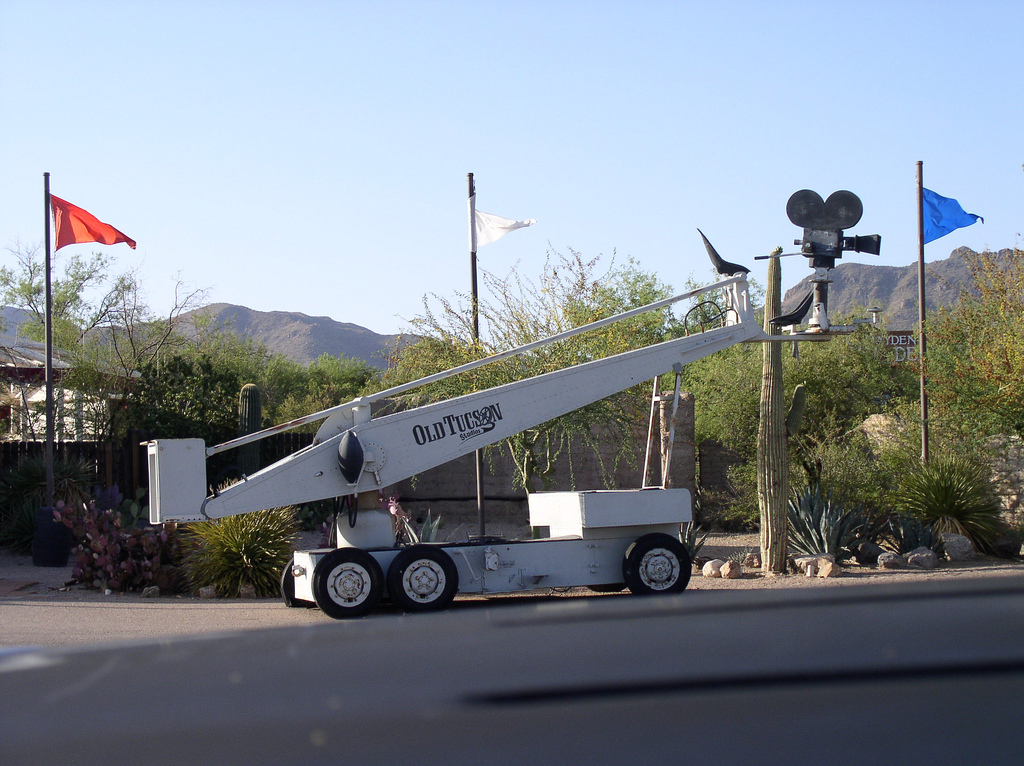
\includegraphics[width=0.49\textwidth]{Bilder/2498906266_844b6be21a_b}}
		\hfill
		\subfloat[Moderner langer Kamerkran]{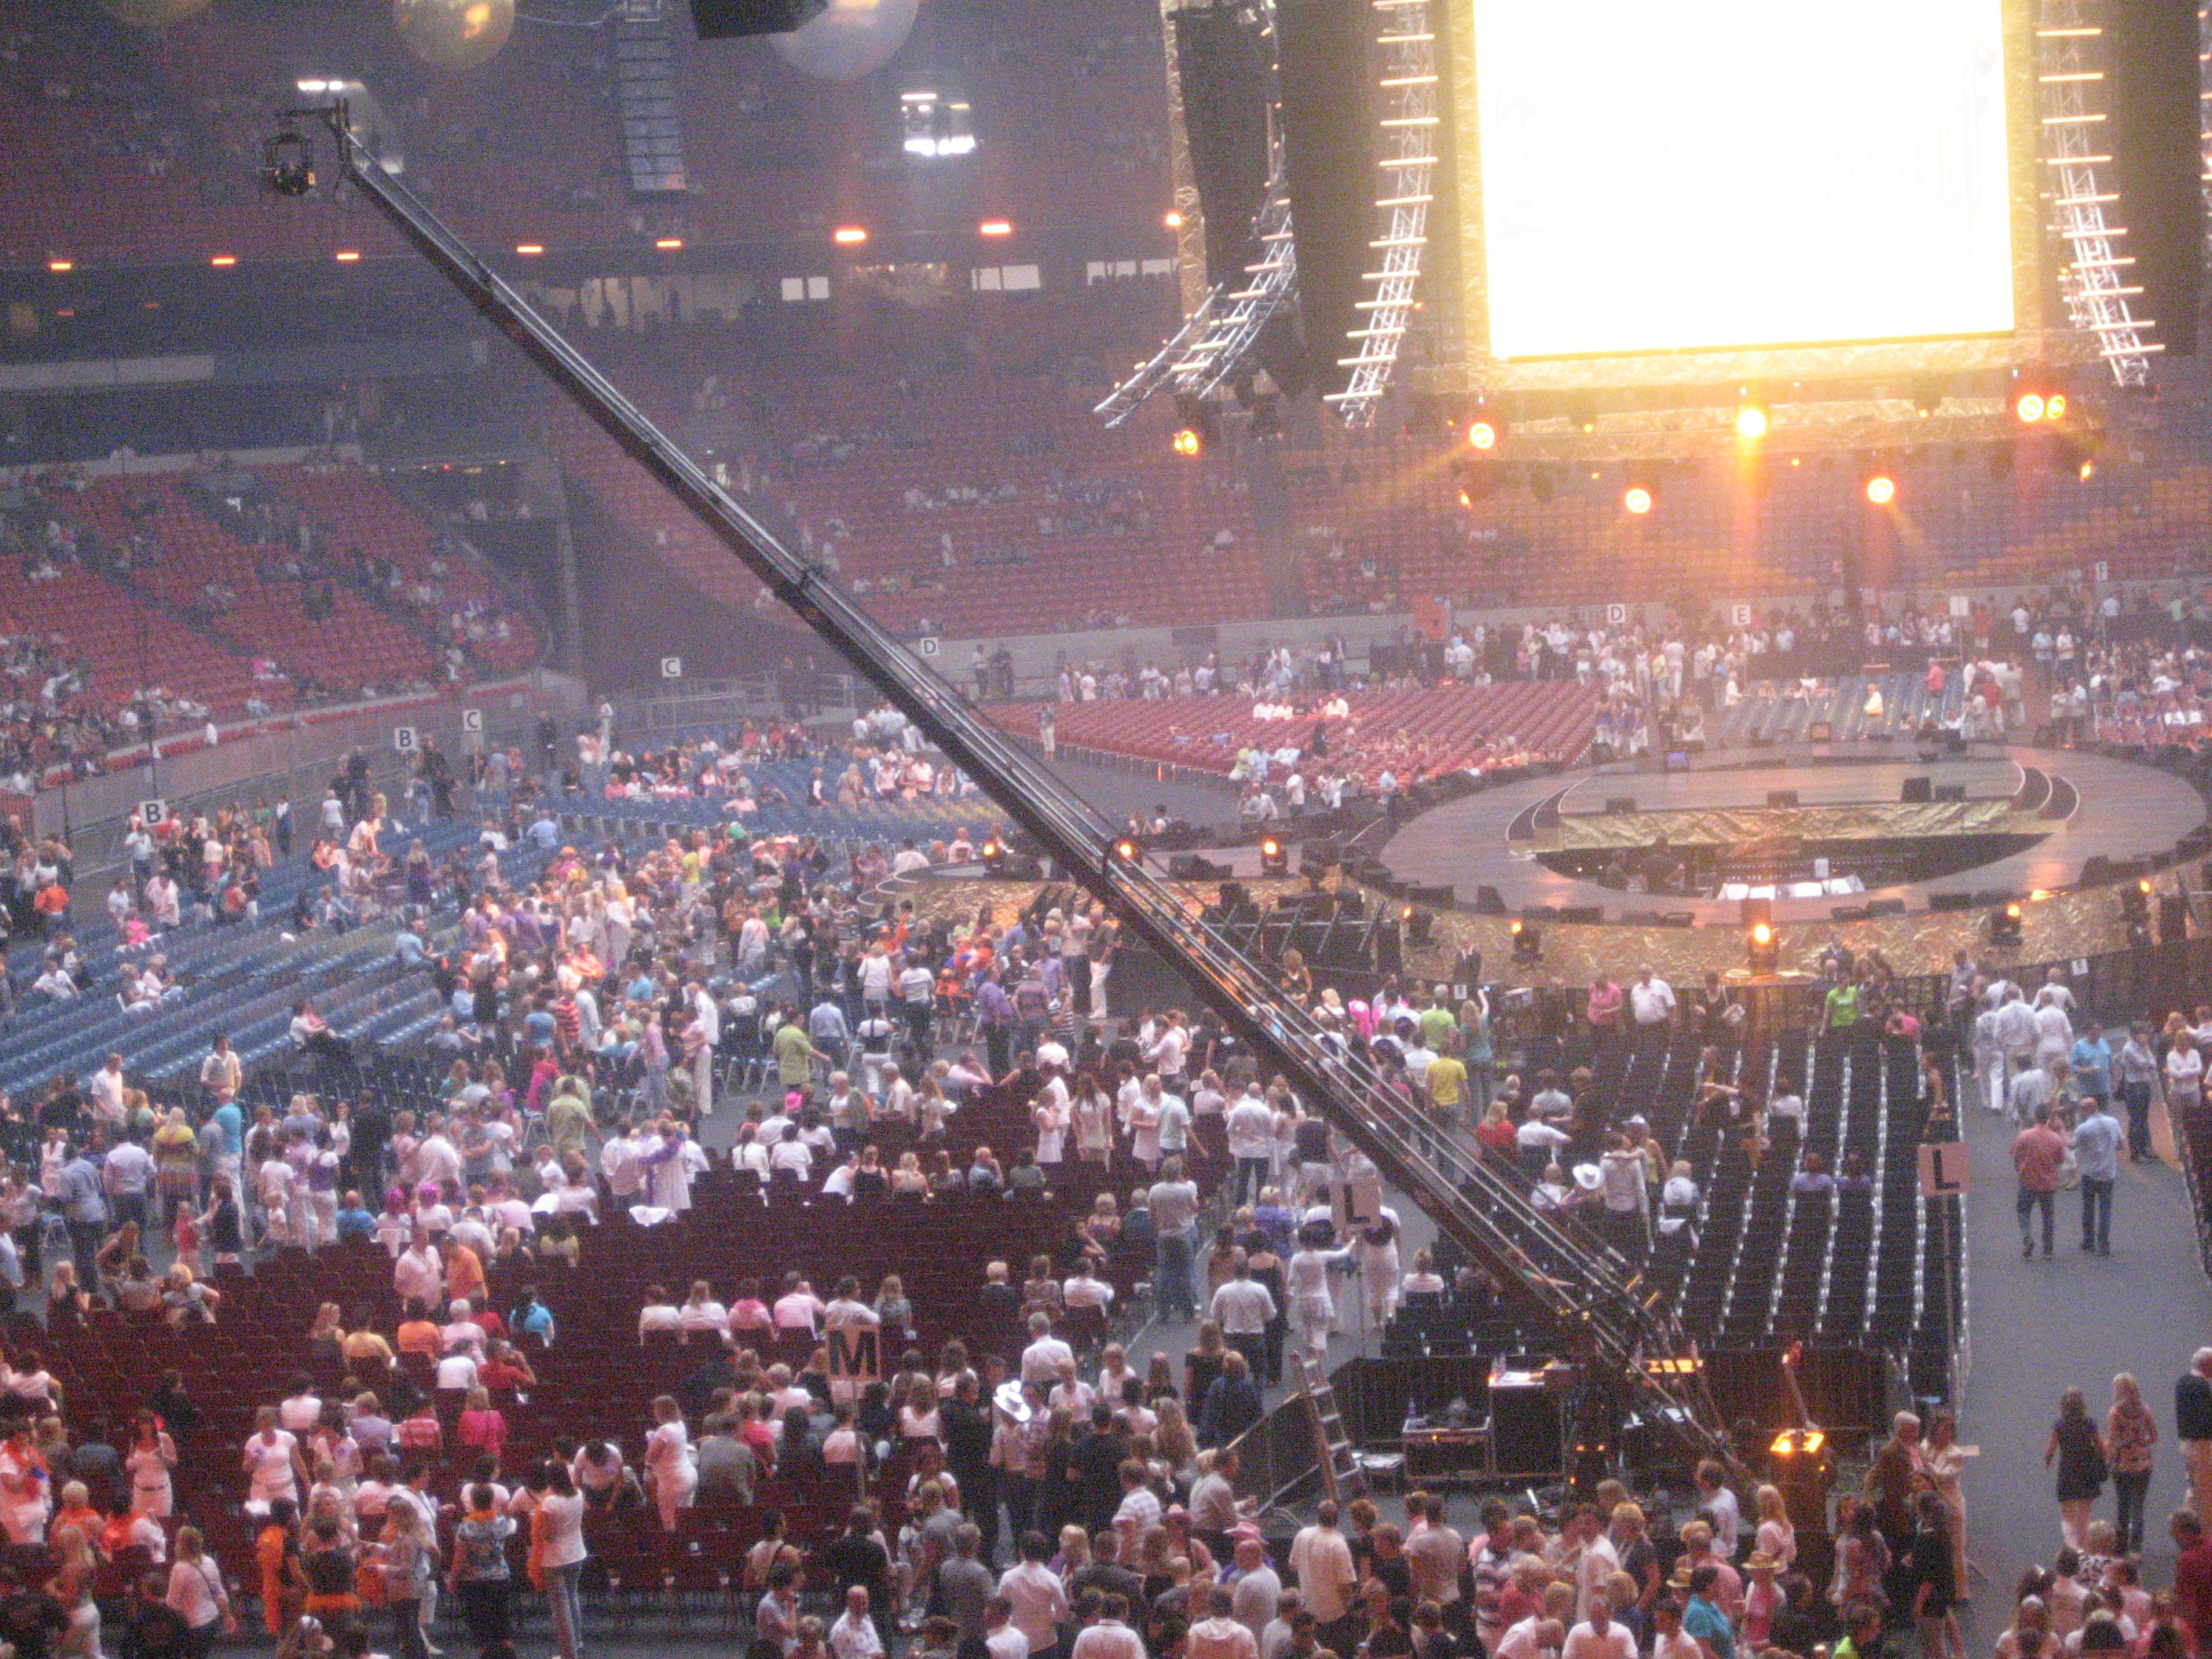
\includegraphics[width=0.49\textwidth]{Bilder/Crane_shot}}
		\caption{Alter und moderner Kamerkran im Vergleich}
	\end{figure}

	Im Wandel der Zeit machten es technische Entwicklungen, besonders im Bereich der Elektrotechnik möglich, die Größe und das Gewicht der Kameras bei etwa gleicher Funktionalität auf ein Minimum zu reduzieren. Zudem ermöglicht die elektronische Steuerung  durch einen Remote-Head die die Fernsteuerung und dadurch ist nicht nur eine weitere Einsparung von Gewicht gegeben, sondern auch eine Vielzahl an Möglichkeiten für die Montage.

	\subsection{Spidercam}
	Die Spidercam (auch unter dem Namen der gleichnamigen Herstellerfirma als “Skycam” bekannt) bezeichnet eine Halterung für Kameras, die üblicherweise durch mehrere Seile an Seilwinden gespannt ist. Durch Verlängern der Seile an einer Winde und gleichzeitiges, synchrones Verkürzen des Seiles an der gegenüberliegenden Winde, kann die Spannung der Seile beibehalten werden und die Halterung so in einer Dimension bewegt werden. Bei der Verwendung mehrerer Seilzüge nach dem gleichen Prinzip, wird auch eine Bewegung in zwei Dimensionen (Ebene) möglich. Dies erfordert jedoch ein Zusammenspiel von synchroner Kontraktion und Relaxion aller Seile an der Halterung der Kamera. Agieren die Seilwinden durch unterschiedlich schnelle, beziehungsweise ungleichmäßige Verlängerung und/oder Verkürzung der Seile gegenläufig, so ist auch eine gleichzeitige Bewegung in der dritten Dimension, der Höhe, möglich. Dabei ist anzumerken, dass man in dieser Dimension, durch die Seile bedingt, üblicherweise nur nach unten fahren kann, da die maximale Höhe, die der gespannten Seile ist. Trotzdem bietet die Spidercam einen großen Vorteil gegenüber gewöhnlichen Kamerakränen, da diese durch die Seilkonstruktion auch bei schwierigem Terrain eingesetzt werden kann und auch besser transportiert werden können. Am häufigsten wird die Spidercam bei Sportveranstaltungen in großen Hallen oder Stadien eingesetzt, da hier der Einsatz von Kamerakränen unvorteilhaft wäre. Für Filmproduktionen ist es aber auch üblich, Kräne zum Spannen der Seile einzusetzen, denn Spidercams ermöglichen auch weite Fahrten.
	
	\begin{figure}[!htb]
		\centering
		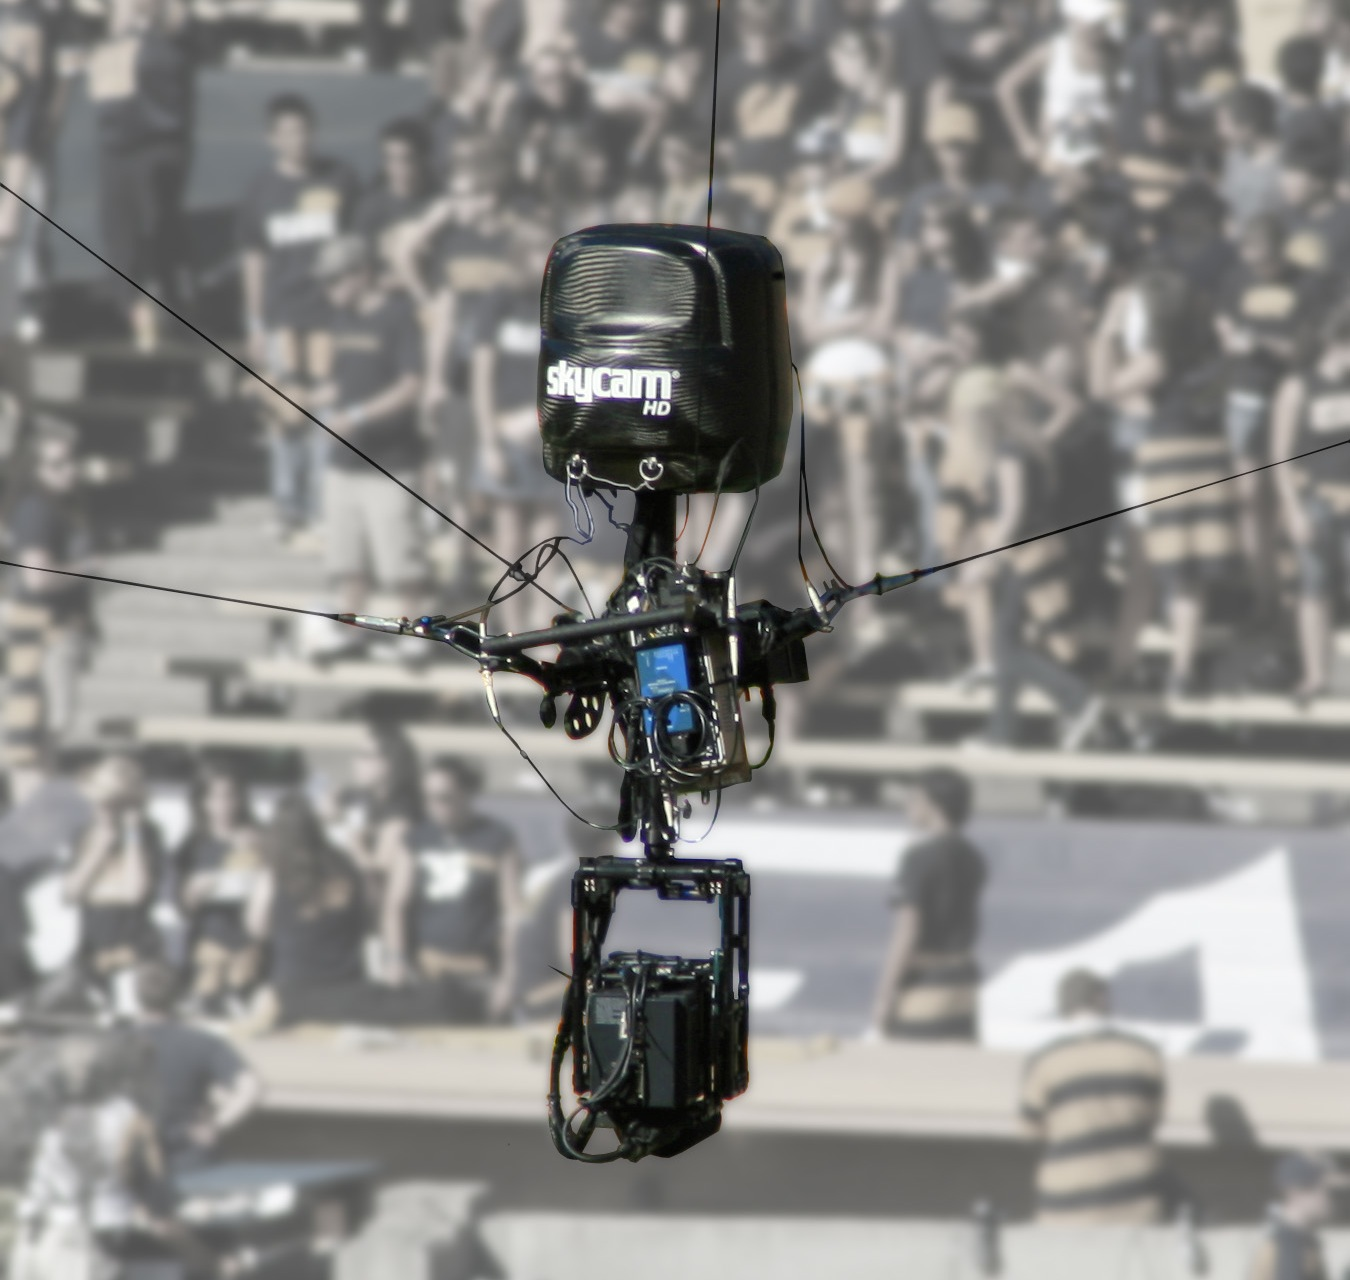
\includegraphics[width=0.5\textwidth]{Bilder/SkycamHDClipEnhanced0346}
		\caption{Eine Spidercam der Firma Skycam bei einer Sportveranstaltung}
	\end{figure}

	\subsection{Seilkamera}
	Als eine Seilkamera werden einzelne oder mehrere parallel gespannte Seile bezeichnet, auf denen ein Schlitten mit der Halterung der Kamera fährt. Dadurch wird es ermöglicht eine lange, eindimensionale Kamerafahrt entlang einer, durch das Seil vorgegebene, Bahn durchzuführen. Seilkameras können von kostengünstigen, einfachen Konstruktionen mit simplen Seilzügen, bis hin zu motorgetriebenen Schlitten variieren.

	\begin{figure}[htb]
		\centering
		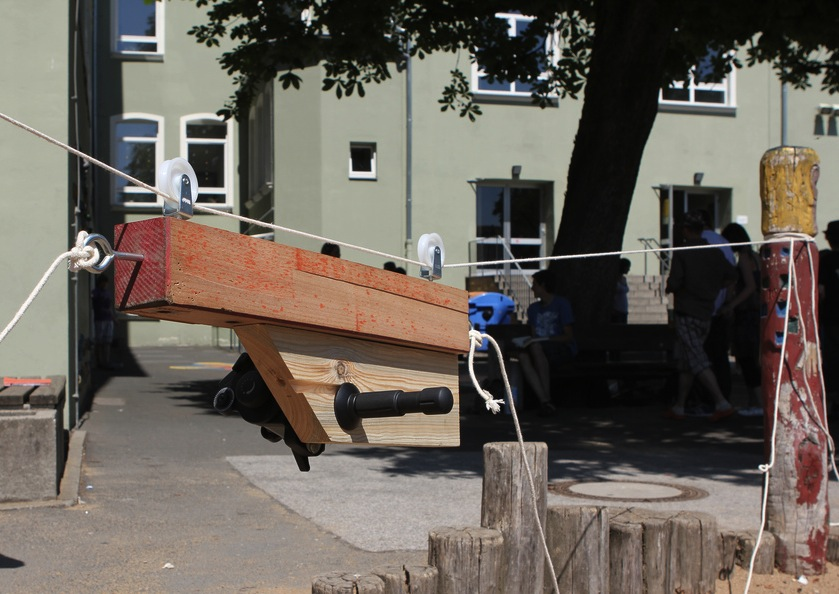
\includegraphics[width=0.8\textwidth]{Bilder/Seilkamera}
		\caption{Einfachste Form einer selbst gebauten Silkamera mit Stativkopf}
	\end{figure}

	\subsection{Helicam}
	Eine Helicam beschreibt ursprünglich den Einsatz von Kameras an Helikopter, denn so werden Filmaufnahmen mit Kamerafahrten über große Distanzen und bei großen Höhen ermöglicht. Die hohen Kosten und der hohe Geräuschpegel bei dem Einsatz vom Hubschraubern stellen jedoch einen enorm großen Nachteil dar. Deshalb haben sich diverse Alternativen entwickelt, zu denen auch die Möglichkeit zählt, einen Remote-Head an einen Heliumballon zu befestigen. Die Vorteile dabei sind, im Gegensatz zu einem Hubschrauber, die extrem geringen Kosten und die absolute Geräuschlosigkeit. Allerdings ist man bei der Kontrolle der Position vollkommen dem Wind ausgesetzt und bei der Steuerung kann man nur zum Boden reichende Seile einsetzen. Diesen Nachteil versuchen andere Alternativen zu kompensieren. “Mit den Fortschritten bei Werkstoffen und Elektronik werden seit einigen Jahren auch ferngesteuerte Modellhubschrauber als „fliegender Kamerakran“ eingesetzt.” Eine Erfindung auf diesem Gebiet stellt der “Quadrocopter” dar. Oft bietet dieser die Fähigkeit automatischer Stabilisierung und findet dadurch auch beim Einsatz als autonome Drohne zunehmend Beliebtheit bei Militär und anderen Institutionen.

	\subsection{Scheinwerfer}
	Das Prinzip des Remote-Heads wird unter dem Namen “Moving Head” ebenfalls in der Lichttechnik eingesetzt. Statt einer Kamera wird hier ein Scheinwerfer ferngesteuert, wobei meist nur eine stationäre Befestigung an Trägern, wie Traversen, gewünscht ist und dadurch die Bewegung des Lichtkegels ermöglicht wird. Solche Systeme werden für Suchscheinwerfer, zum Beispiel auf Schiffen oder Helikopter, eingesetzt. Des Weiteren gibt es in der Unterhaltungsbranche spezielle Varianten für Konzerte, Theater oder Diskotheken, welche über Farbfilter und sog. Gobos verfügen.

	\section{Eintwicklung eines Remote-Heads}
	\subsection{Auswahlkriterien der Bauteile}
	Die Entwicklung des Remote-Heads unterliegt bei der Wahl des Materials verschiedenen Kriterien, die für den Verlauf der Entwicklung von grundlegender Bedeutung sind.

	\subsubsection{Gewicht und Stabilität}
	Dazu gehört, dass die Konstruktion an vielen Stellen kritischen mechanischen Kräften ausgesetzt ist. Aus diesem Grund schränkt das die Auswahl der Materialien ein, denn diese müssen robust sein, aber dennoch leicht genug sein, um die Motoren möglichst wenig zu belasten. Das Material, das diesen Kriterien am besten entspricht, ist Aluminium. In Form von Vierkantrohren bietet es die größtmögliche Steifigkeit bei verhältnismäßig geringem Gewicht

	\subsubsection{Bearbeitung}
	Allerdings lässt sich dieses durch seine Eigenschaften nur schwer verarbeiten, denn das Schweißen ist nur unter speziellem Schutzgas zum Verhindern der Oxidbildung möglich, denn dieses besitzt einen weitaus höheren Schmelzpunkt als Aluminium selbst. Des Weiteren muss der Schweißdraht, entsprechend dem Grundmaterial, ebenfalls aus Aluminium bestehen. Da diese Umstände einen großen Aufwand von speziellen Geräten erfordern, ist es notwendig auf ein anderes Material auszuweichen. In der Praxis hat sich gezeigt, dass identische Vierkantprofile aus Stahl besser zu verarbeiten sind, obwohl diese um einiges mehr an Gewicht haben, aber damit noch im vertretbaren Bereich liegen.

	\subsubsection{Kosten}
	Einen bedeutungsvollen Faktor bei der Auswahl der Bauteile stellen auch die Anschaffungskosten dar. So sind die Kosten von Stahlprofilen wesentlich geringer als die vergleichbarer Aluprofile. Auch die elektronischen Bauteile werden nach ihrem Preis-Leistungs-Verhältnis ausgewählt und werden in der Stückzahl auch aus Gründen der Einfachheit möglichst gering gehalten.

	\subsection{Mechanische Bauteile}
	\subsubsection{Vierkant-Stahlprofile in U-Form}
	Die einfachste Möglichkeit eine Drehung um zwei Achsen gleichzeitig zu ermöglichen, ist zwei ineinander greifende U-Formen um jeweils die Achse, an der sie befestigt sind, zu drehen. Stattdessen ist auch eine L-Form, oder eine in sich geschlossene Form, wie zum Beispiel ein Quader oder Ring, denkbar. Jedoch bietet eine U-Form die beste Kombination von Gewichtsverteilung auf zwei separate Punkte, möglichst wenig Masse und lässt sich dabei gut fertigen.
Zur Fertigung der U-Formen ist es notwendig die Stahlprofile im Rechten Winkel aufeinander zu befestigen. Ein erster Ansatz ist durch jeweils zwei Eisenwinkel an einer Ecke erfolgt, welche mit Bohrungen durch die Stahlprofile für die haltenden Schrauben befestigt waren. Durch die Möglichkeit des Schweißens sind diese im zweiten und endgültigen Ansatz entfallen. Dadurch ergibt sich bei einem Gewicht von jeweils 50g eine Gewichtseinsparung von insgesamt 400g.

	\begin{figure}[htb]
		\centering
		\subfloat[Erster Ansatz mit bereits teilweise entfernten Eisenwinkeln]{\includegraphics[width=0.49\textwidth]{Bilder/IMG_3282}}
		\hfill
		\subfloat[Zweiter, besserer Ansatz]{\includegraphics[width=0.49\textwidth]{Bilder/IMG_3309}}
		\caption{Fertigung der Vierkant-Stahprofile in U-Form}
	\end{figure}

	\subsubsection{Achsen}
	Die Achsen dienen hauptsächlich zur Drehmomentübertragung des Motors auf die U-Formen. Dazu müssen sie mit geeigneten Kupplungen verbunden werden, welche in der Lage sein müssen dem Drehmoment stand zu halten. Eine anfängliche Kupplung konnte durch die ungenügende Sicherung mit Madenschrauben nicht die Kraft übertragen und wurde durch Kupplungen mit Klemmnaben ersetzt. Die verwendete Kupplung hat passend zur Motorwelle einen Lochdurchmesser von 6mm und wird jeweils mit einem 6mm dickem, verschweißten Rundstahl an der U-Form verbunden. Auf der anderen Seite der verbundenen U-Formen werden die Kräfte auf ein identisches Rundstahl verteilt. Dieses lässt sich in das Gewinde des äußeren Stahlprofils schrauben und mit einer Hutmutter sichern und läuft frei in der inneren U-Form

	\begin{figure}[htb]
		\centering
		\includegraphics[width=0.8\textwidth]{Bilder/IMG_3307}
		\caption{Die versenkte Kupplung, verbunden mit der Motorwelle und der festen Achse an der U-Form}
	\end{figure}

	\subsection{Fertigung der Elektrotechnik}
	\subsubsection{Verkabelung}

	\subsubsection{Stromversorgung}

	\subsubsection{Motorsteuerung}
	Zum Wechseln der Drehrichtung beim Gleichstrommotor ist eine elektrische Schaltung zur Umpolung der Spannung notwendig. Realisiert wird dies durch einen so genannten Vierquadrantensteller. Für die Steuerung von Motoren sind bereits Bauteile mit solchen integrierten Schaltungen (IC) erhältlich. Durch ausgiebige Recherche hat sich gezeigt, dass der IC mit der Bezeichnung L298N am besten geeignet ist, denn dieser kann mit nur einem Bauteil zwei Motoren mit einer Spannung von insgesamt 48V und einem Strom von 4A separat ansteuern. Allerdings benötigt dieser integrierte Schaltkreis externe Freilaufdioden. Diese haben die Aufgabe das Bauteil vor der induktiven Gleichspannungslast durch die Elektromotoren zu schützen, denn diese könnte eine permanente Beschädigung des IC hervorrufen.

	\subsubsection{Sensoren}
	Zur Feststellung der aktuellen Position einer U-Form dienen photoelektrische Inkrementalgebe (auch Drehgeber genannt) als Sensoren. Diese bestehen aus einer einer Leuchtdiode, die auf zwei, leicht versetze Fototransistoren gerichtet ist. Eine Encoderscheibe mit mit einem bestimmten Muster von Schlitzen läuft zwischen Diode und Fototransistoren. Bei Rotation der Scheibe durch die Befestigung an der Motorwelle wird das Licht der Diode zu den Fototransistoren regelmäßig unterbrochen und erzeugt so zwei sinusähnliche Signale. Vergleicht man nun die Signale kann durch die gegenseitige Phasenverschiebung die Laufrichtung bestimmt werden. Darüber hinaus kann durch Analyse des Tastgrads eines eingehendes Signals die Geschwindigkeit und der zurückgelegte Winkel an der Encoderscheibe berechnet werden.

	\subsubsection{Mikrocontroller}
	Ein Mikrocontroller ist ein elektronisches Halbleiterbauelement, welches durch einen eingebauten Prozessor und Speicherfunktionen über Rechenleistung zur Signalverarbeitung verfügt. “Ein Mikrocontroller ist praktisch ein Ein-Chip-Computersystem (...) in Leistung und Ausstattung auf die jeweilige Anwendung angepasst.”
	Zur Programmierung eines Mikrocontrollers muss dieser üblicherweise mit einer speziellen Vorrichtung an einen Computer angeschlossen werden und mit der Routine zur Signalverarbeitung programmiert werden. Aufgrund der oft nur sehr knappen Ressourcen ist meist die Programmierung in einer hardwarenahen Programmiersprache notwendig, “um möglichst hohe Effizienz und Code-Dichte zu erreichen.” Nach der Programmierung muss der Mikrocontroller in die eigentliche Schaltung eingesetzt und integriert werden. Damit bildet es meist das zentrale Element einer elektronischen Schaltung, da eingehende Signale durch Sensorik oder ähnlichem ausgewertet werden und die ausgehenden Signale dementsprechend angepasst werden.
	In der Praxis gestaltet sich bereits die Wahl eines Mikroprozessors aus der unermesslichen Fülle von verschieden Komponenten, Architekturen, Bauweisen und ähnlichem sehr schwer. Auch die Anschaffung der Schnittstelle zur Programmierung, die Programmierung selbst und das erneute Ein- und Ausbauen des Mikrocontrollers zur Änderung der Software mit der Routine führt zu einem nicht tragbaren Aufwand und sprengt den Horizont der Arbeit.
	Für die Entwicklung mit Mikrocontrollern gibt es diverse Plattformen, die diesen gesamten Prozess auf ein überschaubares Minimum reduzieren. Durch die weite Verbreitung und einfache Bedienung ist die Wahl auf die flexible, quelloffene Arduino-Plattform gefallen, denn diese bietet durch die gesamte Entwicklungsumgebung “insbesondere Künstlern, Designern, Hobbyisten und anderen Interessierten den Zugang zur Programmierung und zu Mikrocontrollern”.
	Die Serie aus dem Jahr 2009 mit dem Namen Arduino “Duemilanove” (italienisch für “Zweitausendneun”) hat den Anforderungen zur Entwicklung unter der Berücksichtigung des Preis-Leistungsverhältnises am besten entsprochen. Es bietet neben dem Mikroprozessor “ATmega328” mit insgesamt 20 analogen und digitalen Ein- und Ausgängen genügend Anschlussmöglichkeiten für Sensoren und Motorsteuerung.
	Dank der USB-Schnittstelle am Arduino, ist es möglich diesen zu Programmieren und durch Senden und Empfangen von seriellen Signalen in den Programmablauf des Mikrocontrollers einzugreifen.

	\begin{figure}[htb]
		\centering
		\includegraphics[width=0.8\textwidth]{Bilder/Arduino}
		\caption{Arduino Duemilanove}
	\end{figure}

	\subsection{Entwicklung der Software}
	Die Entwicklung der Software für den Controller geschieht in der, als Download verfügbaren, gleichnamigen Entwicklungsumgebung (IDE) “Arduino” unter Zuhilfenahme der verwandten IDE “Processing”, zum Erstellen der Bedieungsoberfläche für die Steuerung des Controllers.
	Die Software des Controllers hat die Aufgabe alle eingehenden Signale der Sensoren und der Steuerung zu interpretieren und dementsprechend die Ausgangssignale für den IC zur Motorsteuerung zu erzeugen.

	\begin{figure}[htb]
		\centering
		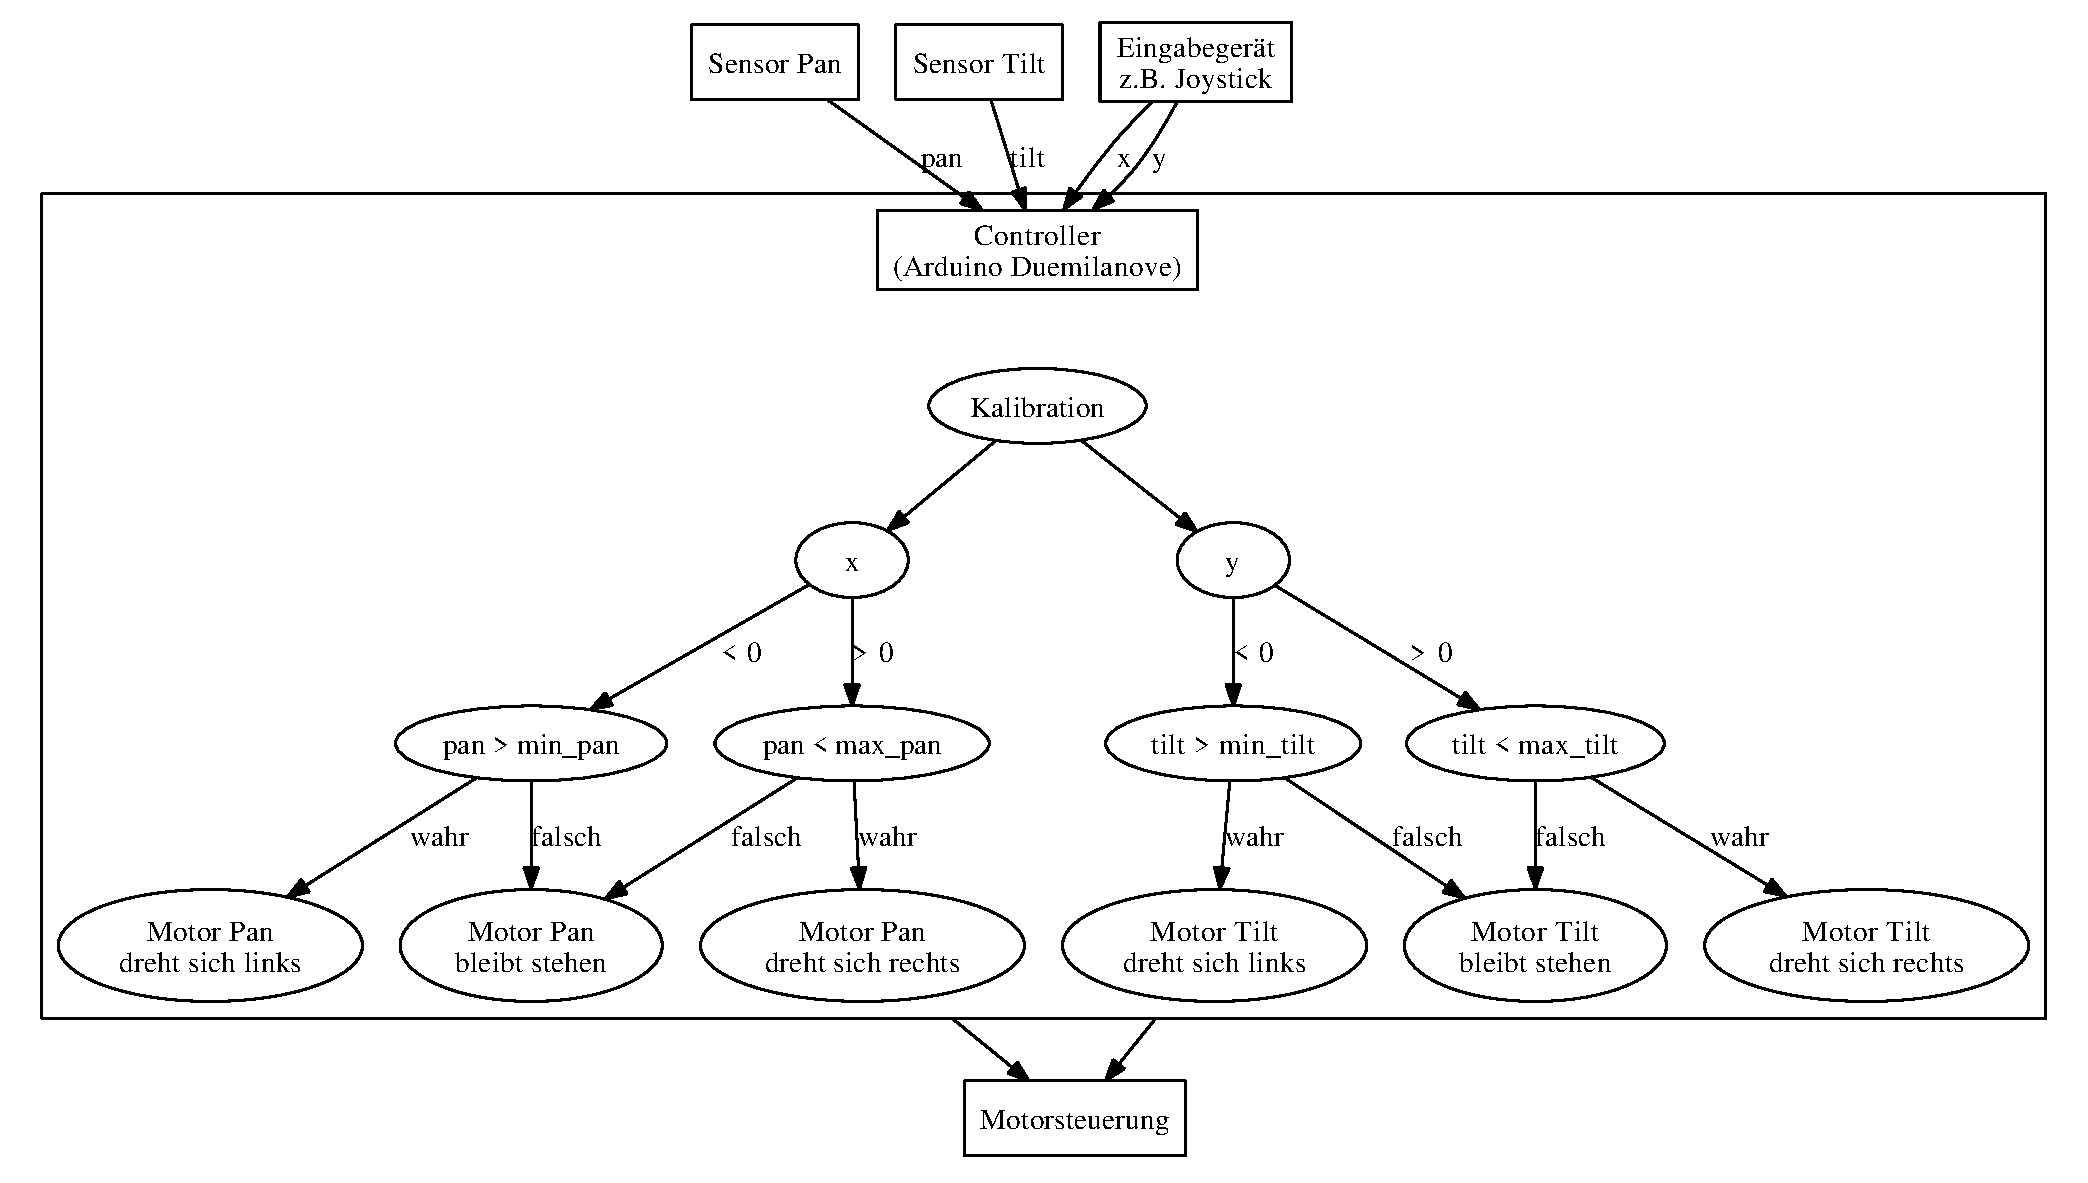
\includegraphics[scale=0.7,angle=90]{Bilder/Programmablaufplan}
		\caption{Programmablaufplan mit der Logik des Programmes}
	\end{figure}

	\section{Bedienung}
	\subsection{Kalibrierung}
	Bei Inbetriebnahme müssen beide U-Formen in die so genannte “Nullstellung” gestellt werden. Dies dient dazu, dass der Controller jede Bewegung auf diesen Punkt beziehen kann und somit ein Anstoßen der Kamera vermieden wird. Von weitaus wichtigerer Bedeutung ist jedoch, dass die Kabel durch einen limitierten Bewegungsbereich nicht verdreht werden können und damit das Entstehen eines Kabelbruchs verhindert werden kann.

	Das Limitieren des Bewegungsbereiches wird durch die Maximalpunkte erreicht. Diese müssen ebenfalls bei Inbetriebnahme kalibriert werden. Dabei ist zu beachten, dass auf beiden Seiten ein unterschiedlicher Bewegungsbereich möglich sein kann.

	\subsection{Steuerung}
	\subsubsection{Eingabegeräte}
	Die Steuerung eines gewöhnlichen Remote-Heads erfolgt üblicherweise durch ein spezielles Eingabegerät, das das gleichzeitige Bedienen beider Achsen ermöglicht. Solche Eingabegeräte können, denen aus dem Modellbau bekannten, Fernbedienungen mit zwei getrennten, einachsigen Joysticks gleichen, aber auch einem zweidimensionalen Joystick für Computer entsprechen. Oft werden auch Trackballs als Eingaberäte verwendet. Prinzipiell sind alle Eingabegeräte mit vielen Stufen zur Steuerung denkbar und so lassen sich auch Potentiometer oder Mäuse zur Steuerung nutzen.

	\subsubsection{Computer}
	Die Steuerung per Computer wird durch die am Controller befindliche USB-Schnittstelle möglich. Dabei stellt das Programm eine simulierte serielle Verbindung auf. Alternativ kann das Board aufgrund dessen Erweiterbarkeit durch eine kabellose Methode gesteuert werden, indem man ein entsprechendes Modul (z.B. “XBee Shield”) verwendet. Gleichgültig der Schnittstelle agiert das Programm immer auf die gleiche Weise und ermöglicht es die Manöver an den Controller zu senden. Vorteile in Verwendung mit einen Computer bestehen zum einen darin, dass angeschlossene Peripherie, wie zum Beispiel ein Joystick, zum Bedienen des Remote-Heads verwendet werden können. Ein weiterer Vorteil ist aber auch, dass je nach Verwendung der Kamera auch deren Vorschaubild über eine zusätzliche Leitung übertragen werden kann. Beispielsweise stehen bei einer Canon EOS 550D zwei Schnittstellen zur Auswahl: HDMI und ein entsprechender Anschluss für analoge Bildübertragung per Composite. Der Vorteil einer solchen Bildübertragung besteht darin, dass das Bildmaterial schon während der Aufnahme zur Kontrolle abgenommen und auch gespeichert werden kann.

	\section{Fazit}
	Ein Remote-Head kann über ein großes Spektrum von Einsatzmöglichkeiten verwendet werden. In vielen Bereichen, wie zum Beispiel in der Überwachungstechnik in Verkehr und Sicherheit, Militär, der Unterhaltungsbranche bei Konzerten, Diskotheken und natürlich auch in der Filmbranche, ist diese Technologie nicht mehr wegzudenken.  Abhängig von den räumlichen Gegebenheiten, dem Verwendungszweck und zuletzt dem Budget variieren die verschiedenen Anwendungen. Dass solche Systeme nicht immer teuer sein müssen und es neben den sehr leistungsfähigen kommerziellen Systemen auch möglich ist, sich mit einem gewissen Maß an Fachkenntnissen, der notwendigen Einarbeitungszeit und den geeigneten Mitteln, einen eigenen, auf die eigenen Bedürfnisse angepassten, Remote-Head zu entwickeln, hat diese Facharbeit bewiesen. Bei dieser Entwicklung eines Remote-Heads für einen Kamerakran haben sich einige Schwierigkeiten bei der Planung der mechanischen Konstruktion durch die Einbeziehung aller Teile gezeigt, denn diese musste im Lauf der Entwicklung oft angepasst werden. Zudem Bedarf die Elektronik einer ausgiebigen Einarbeitung und fordert vom Entwurf bis hin zur fertigen Schaltung. Schon mit dem Verständnis der elektronischen Schaltung lässt sich die Software zur Steuerung schematisch entwerfen und mit Referenzen aus Internet und der Dokumentation vervollständigen.

	\pagebreak

	% Bibliographie
	% Um die Bibliographie einzubinden sind folgende Schritte notwendig:
	% 1. LaTeX setzen (findet NOTWENDIGE Verweise und speichert diese in .aux-Datei)
	% 2. BibTeX setzen (generiert .bbl-Datei)
	% 3. LaTeX erneut setzen (bindet .bbl-Datei in das Dokument ein)
	% 4. LaTeX ein weiteres mal setzen
	\nocite{*}
	\bibliography{Quellen}
	\bibliographystyle{natdin}

	% Bilderverzeichnis
	\listoffigures
	\listsubcaptions

	\pagebreak

	% Erklärung
	\section*{Erklärung}
	Ich erkläre, dass ich die Facharbeit ohne fremde Hilfe angefertigt und nur die im Literaturverzeichnis angeführten Quellen und Hilfsmittel benutzt habe.\\
	\\
	\\
	\begin{minipage}{3cm}
		..................................,\\
		\it{Ort}
	\end{minipage}
	\hspace{1.5cm}
	\begin{minipage}{2cm}
		...........................\\
		\it{Datum}
	\end{minipage}
	\hspace{1.5cm}
	\begin{minipage}{8cm}
		.........................................................\\
		\it{Unterschrift des Schülers}
	\end{minipage}
\end{document}